\documentclass[12pt]{extarticle}

\usepackage[color=red]{todonotes}
\usepackage{mathtools}
\usepackage{algorithmic}
\usepackage{amsfonts}
\usepackage{pdflscape}
\usepackage{graphicx}
\usepackage{listings}
\usepackage{subfig}
\usepackage{enumitem}

\usepackage{lscape}
\usepackage{longtable}

\usepackage{savesym}
\savesymbol{newfloat}
\usepackage{floatrow}
\restoresymbol{TXF}{newfloat}

\begin{document}

\title{Visualization}
\date{}
\author{}
\maketitle
\noindent
This example shows a setting of a world with two inspection locations. The drone initially takes off at Home. It succeeds in inspecting the first location, but on its way to the second location, the policy decides upon returning Home (due to low battery). In this scenario, the overall goal was not reached (as not all inspection locations are inspected), but the drone did reach Home again safely.\\
First we show the output model (i.e. an instantiation of the structure), followed by the visualization itself.
\subsubsection*{Output Model}
\begin{lstlisting}[basicstyle=\tiny]
structure  : V {
  Distance = { 0..3 }
  FlyHeight = { 3..4 }
  GroundHeight = { 0..0 }
  Height = { 0..5 }
  Inspection = { Insp1; Insp2 }
  InspectionHeight = { 1..2 }
  Power = { 0..100 }
  PowerUsage = { 0..5 }
  RestrictedHeight = { 5..5 }
  Time = { 0..40 }
  AllPicturesTaken = {  }
  AtCriticalPower = { 34; 35; 36; 37; 38; 39; 40 }
  AtFlyHeight = { 5; 6; 7; 8; 9; 10; 14; 15; 16; 17; 18; 19; 20; 21; 22; 23 }
  AtGroundHeight = { 0; 1; 26; 27; 28; 29; 30; 31; 32; 33; 34; 35; 36; 37; 38; 39; 40 }
  AtHome = { 0; 1; 2; 3; 4; 5; 23; 24; 25; 26; 27; 28; 29; 30; 31; 32; 33; 34; 35; 36;
             37; 38; 39; 40 }
  AtInspection = { 10; 11; 12; 13; 14; 15; 16; 17 }
  AtInspectionHeight = { 2; 3; 4; 11; 12; 13; 24; 25 }
  AtInspectionToDo = { 10; 11 }
  AtLowPower = { 18; 19; 20; 21; 22; 23; 24; 25; 26; 27; 28; 29; 30; 31; 32; 33; 34;
                 35; 36; 37; 38; 39; 40 }
  AtNormalPower = { 0; 1; 2; 3; 4; 5; 6; 7; 8; 9; 10; 11; 12; 13; 14; 15; 16; 17 }
  AtRestrictedHeight = {  }
  AtTravelSpace = { 6; 7; 8; 9; 18; 19; 20; 21; 22 }
  CN_DistanceToHome = { 5,0; 5,2; 5,3; 17,0; 17,1; 17,2; 18,0; 18,1; 18,3; 20,0;
                        20,2; 20,3 }
  CN_DistanceToRA = { 5,0; 5,2; 5,3; 7,0; 7,1; 7,3; 9,0; 9,2; 9,3; 15,0; 15,1;
                      15,3; 18,0; 18,2; 18,3; 19,0; 19,1; 19,3 }
  CN_DistanceToTarget = { 5,0; 5,2; 5,3; 17,0; 17,1; 17,2; 18,0; 18,1; 18,3;
                          20,0; 20,2; 20,3 }
  CN_Height = { 1,0; 1,2; 1,3; 1,4; 1,5; 3,0; 3,1; 3,3; 3,4; 3,5; 4,0; 4,1; 4,2;
                4,4; 4,5; 10,0; 10,1; 10,3; 10,4; 10,5; 13,0; 13,1; 13,2; 13,4;
                13,5; 23,0; 23,1; 23,3; 23,4; 23,5; 24,0; 24,2; 24,3; 24,4; 24,5;
                25,1; 25,2; 25,3; 25,4; 25,5 }
  
  
  CN_Location = { 5,Home; 5,Insp1; 5,Insp2; 5,Insp3; 5,Insp4; 9,Home; 9,Insp2;
                  9,Insp3; 9,Insp4; 9,TravelSpace; 17,Home; 17,Insp1; 17,Insp2;
                  17,Insp3; 17,Insp4; 22,Insp1; 22,Insp2; 22,Insp3; 22,Insp4;
                  22,TravelSpace }
  C_DistanceToHome = { 5,1; 17,3; 18,2; 20,1 }
  C_DistanceToRA = { 5,1; 7,2; 9,1; 15,2; 18,1; 19,2 }
  C_DistanceToTarget = { 5,1; 17,3; 18,2; 20,1 }
  C_Height = { 1,1; 3,2; 4,3; 10,2; 13,3; 23,2; 24,1; 25,0 }
  C_Location = { 5,TravelSpace; 9,Insp1; 17,TravelSpace; 22,Home }
  C_Picture_Taken = { 11,Insp1 }
  CloseToRA = { 6; 7; 10; 11; 12; 13; 14; 15; 19 }
  NonDetDecreaseDistRA = { 5; 9; 18 }
  NonDetIncreaseDistRA = {  }
  NonDetMove = { 1; 3; 4; 5; 7; 9; 10; 11; 13; 15; 17; 18; 19; 20; 22; 23; 24; 25;
                 26; 27; 28; 29; 30; 31; 32; 33; 34; 35; 36; 37; 38; 39; 40 }
  Picture_Taken = { 12,Insp1; 13,Insp1; 14,Insp1; 15,Insp1; 16,Insp1; 17,Insp1;
                    18,Insp1; 19,Insp1; 20,Insp1; 21,Insp1; 22,Insp1; 23,Insp1;
                    24,Insp1; 25,Insp1; 26,Insp1; 27,Insp1; 28,Insp1; 29,Insp1; 
                    30,Insp1; 31,Insp1; 32,Insp1; 33,Insp1; 34,Insp1; 35,Insp1;
                    36,Insp1; 37,Insp1; 38,Insp1; 39,Insp1; 40,Insp1 }
  BackLoopTime = 0
  Battery = { 0->100; 1->95; 2->90; 3->85; 4->80; 5->75; 6->72; 7->69; 8->66;
              9->63; 10->60; 11->58; 12->56; 13->51; 14->46; 15->43; 16->40;
              17->37; 18->34; 19->31; 20->28; 21->25; 22->22; 23->19; 24->17;
              25->15; 26->13; 27->12; 28->11; 29->10; 30->9; 31->8; 32->7; 33->6;
              34->5; 35->4; 36->3; 37->2; 38->1; 39->0; 40->0 }
  Battery_Init = 100
  ClosestInspectionLocationToDo = 
    { 0->Insp1; 1->Insp1; 2->Insp1; 3->Insp1; 4->Insp1; 5->Insp1; 6->Insp1;
    7->Insp1; 8->Insp1; 9->Insp1; 10->Insp1; 11->Insp1; 12->Insp2; 13->Insp2;
    14->Insp2; 15->Insp2; 16->Insp2; 17->Insp2; 18->Insp2; 19->Insp2; 20->Insp2;
    21->Insp2; 22->Insp2; 23->Insp2; 24->Insp2; 25->Insp2; 26->Insp2; 27->Insp2;
    28->Insp2; 29->Insp2; 30->Insp2; 31->Insp2; 32->Insp2; 33->Insp2; 34->Insp2;
    35->Insp2; 36->Insp2; 37->Insp2; 38->Insp2; 39->Insp2; 40->Insp2 }
  CriticalPower = 5
  Curr_DistanceToHome = { 0->0; 1->0; 2->0; 3->0; 4->0; 5->0; 6->1; 7->1; 8->1;
                          9->1; 10->2; 11->2; 12->2; 13->2; 14->2; 15->2; 16->2;
                          17->2; 18->3; 19->2; 20->2; 21->1; 22->1; 23->0; 24->0;
                          25->0; 26->0; 27->0; 28->0; 29->0; 30->0; 31->0; 32->0;
                          33->0; 34->0; 35->0; 36->0; 37->0; 38->0; 39->0; 40->0 }
  Curr_DistanceToRA = { 0->2; 1->2; 2->2; 3->2; 4->2; 5->2; 6->1; 7->1; 8->2;
                        9->2; 10->1; 11->1; 12->1; 13->1; 14->1; 15->1; 16->2;
                        17->2; 18->2; 19->1; 20->2; 21->2; 22->2; 23->2; 24->2;
                        25->2; 26->2; 27->2; 28->2; 29->2; 30->2; 31->2; 32->2;
                        33->2; 34->2; 35->2; 36->2; 37->2; 38->2; 39->2; 40->2 }
  Curr_DistanceToTarget = { 0->2; 1->2; 2->2; 3->2; 4->2; 5->2; 6->1; 7->1; 8->1;
                            9->1; 10->0; 11->0; 12->2; 13->2; 14->2; 15->2; 16->2;
                            17->2; 18->3; 19->2; 20->2; 21->1; 22->1; 23->0; 24->0;
                            25->0; 26->0; 27->0; 28->0; 29->0; 30->0; 31->0; 32->0;
                            33->0; 34->0; 35->0; 36->0; 37->0; 38->0; 39->0; 40->0 }
  Curr_Height = { 0->0; 1->0; 2->1; 3->1; 4->2; 5->3; 6->3; 7->3; 8->3; 9->3;
                  10->3; 11->2; 12->2; 13->2; 14->3; 15->3; 16->3; 17->3; 18->3;
                  19->3; 20->3; 21->3; 22->3; 23->3; 24->2; 25->1; 26->0; 27->0;
                  28->0; 29->0; 30->0; 31->0; 32->0; 33->0; 34->0; 35->0; 36->0;
                  37->0; 38->0; 39->0; 40->0 }
  Curr_Location = { 0->Home; 1->Home; 2->Home; 3->Home; 4->Home; 5->Home;
                    6->TravelSpace; 7->TravelSpace; 8->TravelSpace; 9->TravelSpace;
                    10->Insp1; 11->Insp1; 12->Insp1; 13->Insp1; 14->Insp1;
                    15->Insp1; 16->Insp1; 17->Insp1; 18->TravelSpace;
                    19->TravelSpace; 20->TravelSpace; 21->TravelSpace;
                    22->TravelSpace; 23->Home; 24->Home; 25->Home; 26->Home;
                    27->Home; 28->Home; 29->Home; 30->Home; 31->Home; 32->Home;
                    33->Home; 34->Home; 35->Home; 36->Home; 37->Home; 38->Home;
                    39->Home; 40->Home }
  DistanceBetween = { Home,Home->0; Home,Insp1->2; Home,Insp2->3; Insp1,Home->2;
                      Insp1,Insp1->0; Insp1,Insp2->2; Insp2,Home->3;
                      Insp2,Insp1->2; Insp2,Insp2->0 }
  InitialRestrictedDistance = 2
  LiftPower = 5
  LowPower = { 0->19; 1->19; 2->19; 3->19; 4->19; 5->19; 6->25; 7->25; 8->25; 
               9->25; 10->31; 11->31; 12->31; 13->31; 14->31; 15->31; 16->31;
               17->31; 18->37; 19->31; 20->31; 21->25; 22->25; 23->19; 24->19;
               25->19; 26->19; 27->19; 28->19; 29->19; 30->19; 31->19; 32->19;
               33->19; 34->19; 35->19; 36->19; 37->19; 38->19; 39->19; 40->19 }
  LowerPower = 2
  MoveToPower = 3
  
  Next = { 0->1; 1->2; 2->3; 3->4; 4->5; 5->6; 6->7; 7->8; 8->9; 9->10; 10->11;
           11->12; 12->13; 13->14; 14->15; 15->16; 16->17; 17->18; 18->19; 19->20;
           20->21; 21->22; 22->23; 23->24; 24->25; 25->26; 26->27; 27->28; 28->29;
           29->30; 30->31; 31->32; 32->33; 33->34; 34->35; 35->36; 36->37; 37->38;
           38->39; 39->40 }
  NoOpPower = 1
  Plan = { 0->Lift; 1->Lift; 2->Lift; 3->Lift; 4->Lift; 5->MoveTowardsTarget;
           6->MoveAwayFromRA; 7->MoveAwayFromRA; 8->MoveTowardsTarget;
           9->MoveTowardsTarget; 10->Lower; 11->TakePicture; 12->Lift; 13->Lift;
           14->MoveAwayFromRA; 15->MoveAwayFromRA; 16->MoveTowardsTarget;
           17->MoveTowardsTarget; 18->MoveTowardsTarget; 19->MoveAwayFromRA;
           20->MoveTowardsTarget; 21->MoveTowardsTarget; 22->MoveTowardsTarget;
           23->Lower; 24->Lower; 25->Lower; 26->NoOp; 27->NoOp; 28->NoOp; 29->NoOp;
           30->NoOp; 31->NoOp; 32->NoOp; 33->NoOp; 34->NoOp; 35->NoOp; 36->NoOp;
           37->NoOp; 38->NoOp; 39->NoOp; 40->NoOp }
  PowerUsageAt = { 0->5; 1->5; 2->5; 3->5; 4->5; 5->3; 6->3; 7->3; 8->3; 9->3;
                   10->2; 11->2; 12->5; 13->5; 14->3; 15->3; 16->3; 17->3; 18->3;
                   19->3; 20->3; 21->3; 22->3; 23->2; 24->2; 25->2; 26->1; 27->1;
                   28->1; 29->1; 30->1; 31->1; 32->1; 33->1; 34->1; 35->1; 36->1;
                   37->1; 38->1; 39->0; 40->0 }
  Start = 0
  StaticLowPower = 5
  TakePicturePower = 2
  Target = { 0->Insp1; 1->Insp1; 2->Insp1; 3->Insp1; 4->Insp1; 5->Insp1; 6->Insp1;
             7->Insp1; 8->Insp1; 9->Insp1; 10->Insp1; 11->Insp1; 12->Insp2;
             13->Insp2; 14->Insp2; 15->Insp2; 16->Insp2; 17->Insp2; 18->Home;
             19->Home; 20->Home; 21->Home; 22->Home; 23->Home; 24->Home;
             25->Home; 26->Home; 27->Home; 28->Home; 29->Home; 30->Home;
             31->Home; 32->Home; 33->Home; 34->Home; 35->Home; 36->Home;
             37->Home; 38->Home; 39->Home; 40->Home }
  Weight = 1
}
\end{lstlisting}

\vspace{10mm}

\subsubsection*{Visualization}
The visualization can be ran by executing the command
\begin{center}
    \textit{Vis\textbackslash main.py normal\_flight}.
\end{center}
The individual titles of the following plots (starting at the next page) indicate the planned action at the corresponding time step. This action is supposedly executed during the succession of the current time step to the next one. The color of the title denotes whether or not the action was successful. A green title indicates a successful action, a red title indicates a failed attempt. The symbols on the plots represent the Locations, as indicated in the legend. The first 30 time steps are shown. After time step 26, the drone remains landed at home, draining the battery under normal operation (of communication etc.).
\clearpage
\begin{figure}[!htb]
  \centering
  \subfloat{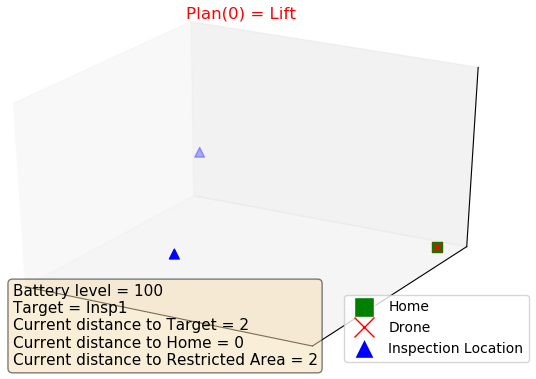
\includegraphics[width=0.5\textwidth]{plots/plt0}}
  \subfloat{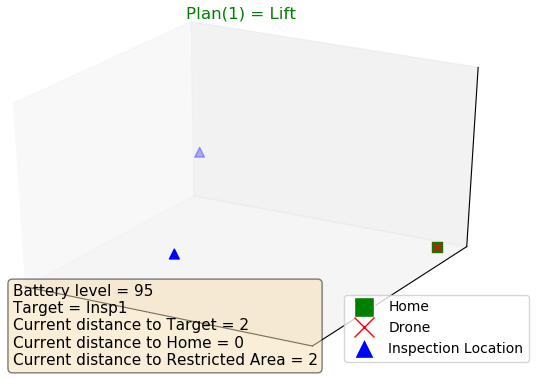
\includegraphics[width=0.5\textwidth]{plots/plt1}}
\end{figure}
\begin{figure}[!htb]
  \centering
  \subfloat{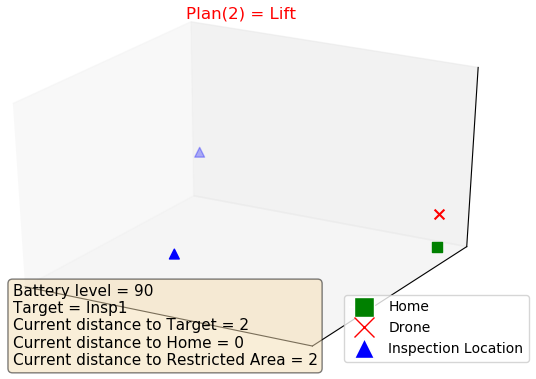
\includegraphics[width=0.5\textwidth]{plots/plt2}}
  \subfloat{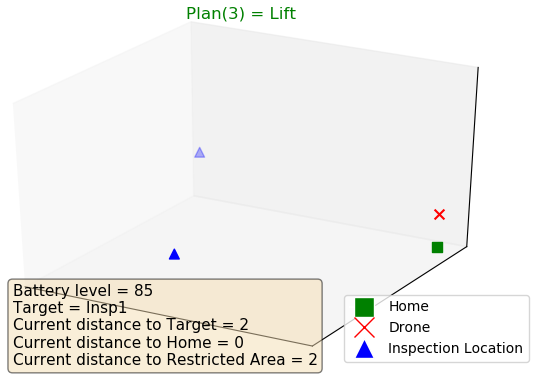
\includegraphics[width=0.5\textwidth]{plots/plt3}}
\end{figure}
\begin{figure}[!htb]
  \centering
  \subfloat{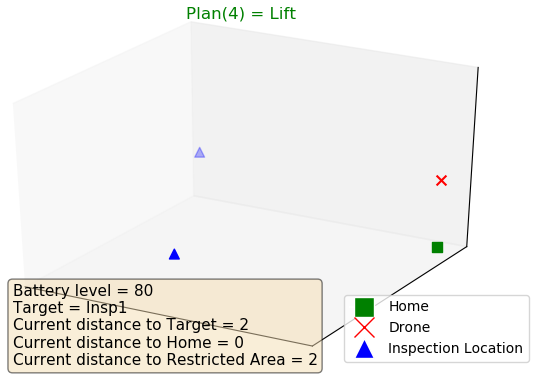
\includegraphics[width=0.5\textwidth]{plots/plt4}}
  \subfloat{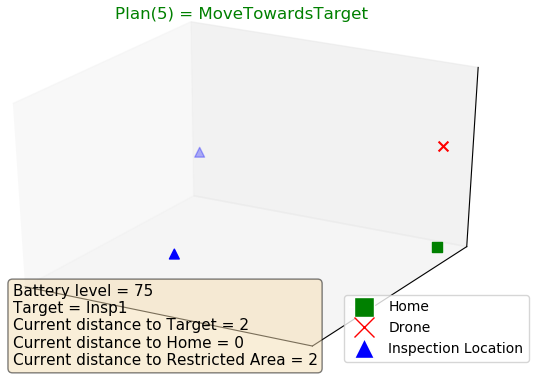
\includegraphics[width=0.5\textwidth]{plots/plt5}}
\end{figure}
\begin{figure}[!htb]
  \centering
  \subfloat{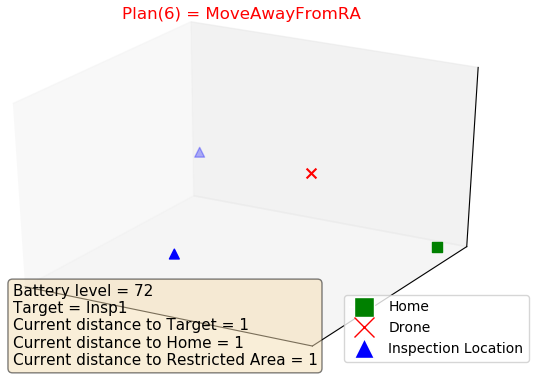
\includegraphics[width=0.5\textwidth]{plots/plt6}}
  \subfloat{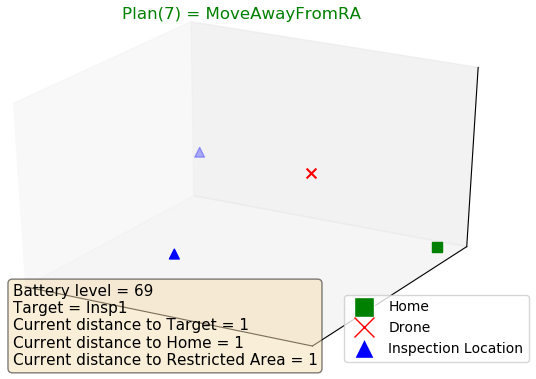
\includegraphics[width=0.5\textwidth]{plots/plt7}}
\end{figure}
\begin{figure}[!htb]
  \centering
  \subfloat{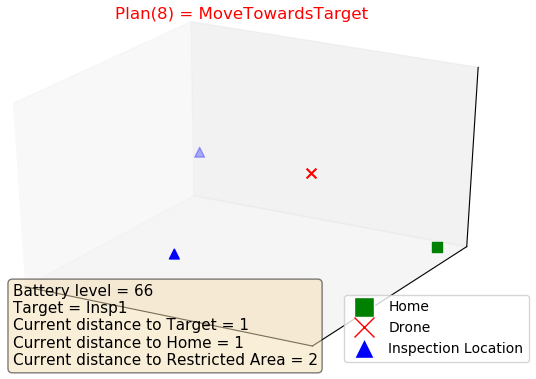
\includegraphics[width=0.5\textwidth]{plots/plt8}}
  \subfloat{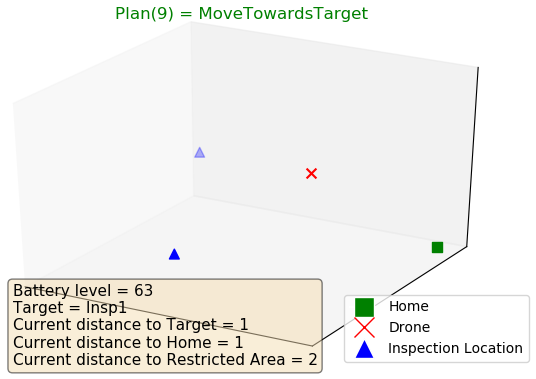
\includegraphics[width=0.5\textwidth]{plots/plt9}}
\end{figure}
\begin{figure}[!htb]
  \centering
  \subfloat{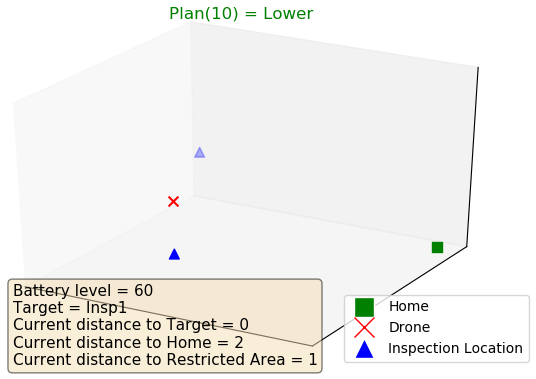
\includegraphics[width=0.5\textwidth]{plots/plt10}}
  \subfloat{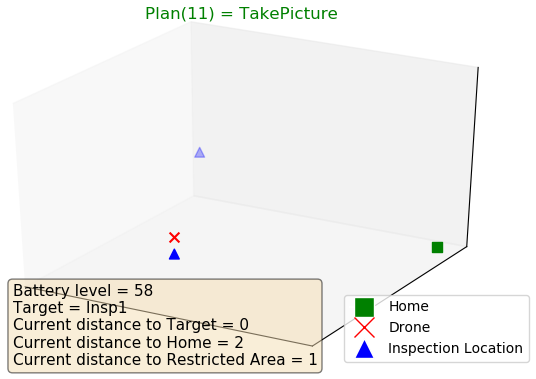
\includegraphics[width=0.5\textwidth]{plots/plt11}}
\end{figure}
\begin{figure}[!htb]
  \centering
  \subfloat{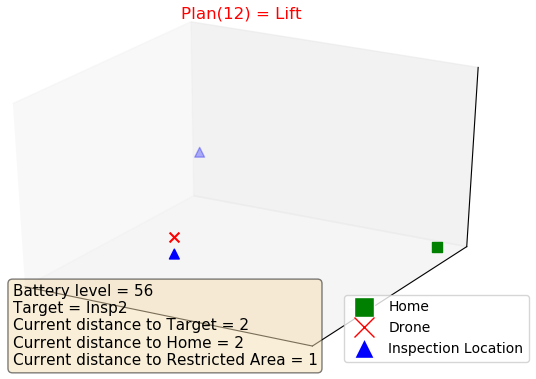
\includegraphics[width=0.5\textwidth]{plots/plt12}}
  \subfloat{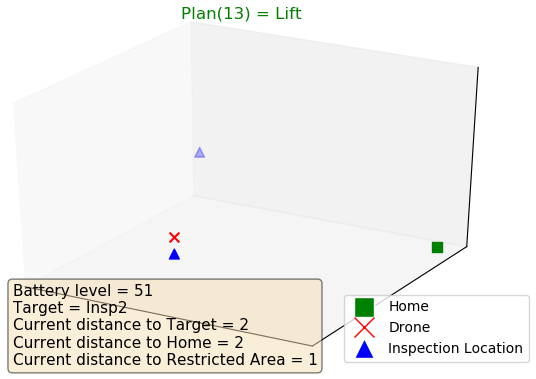
\includegraphics[width=0.5\textwidth]{plots/plt13}}
\end{figure}
\begin{figure}[!htb]
  \centering
  \subfloat{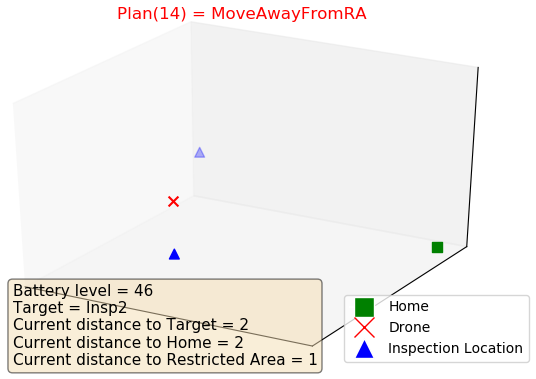
\includegraphics[width=0.5\textwidth]{plots/plt14}}
  \subfloat{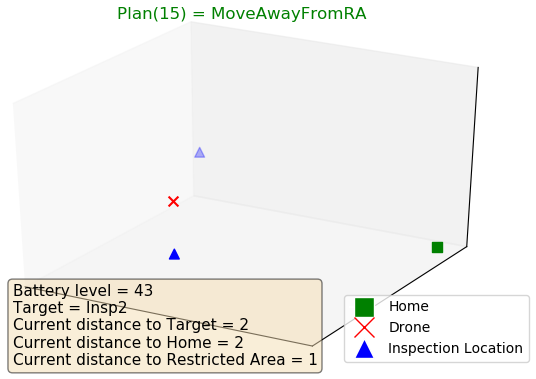
\includegraphics[width=0.5\textwidth]{plots/plt15}}
\end{figure}
\begin{figure}[!htb]
  \centering
  \subfloat{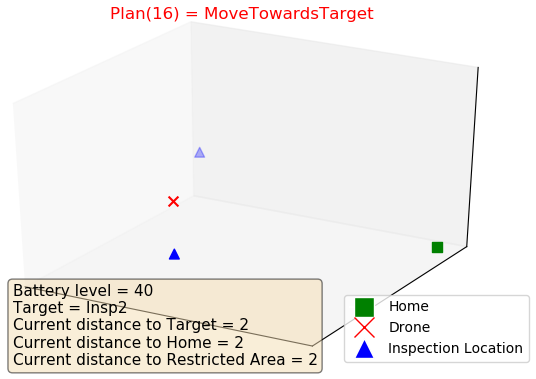
\includegraphics[width=0.5\textwidth]{plots/plt16}}
  \subfloat{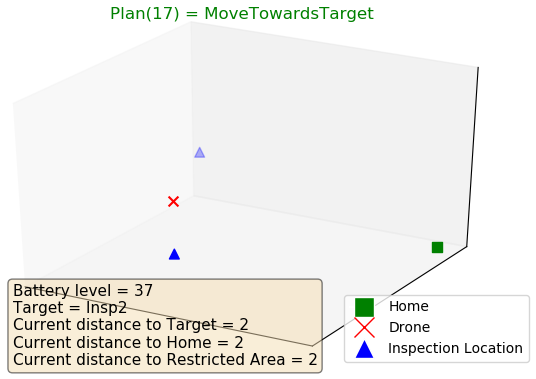
\includegraphics[width=0.5\textwidth]{plots/plt17}}
\end{figure}
\begin{figure}[!htb]
  \centering
  \subfloat{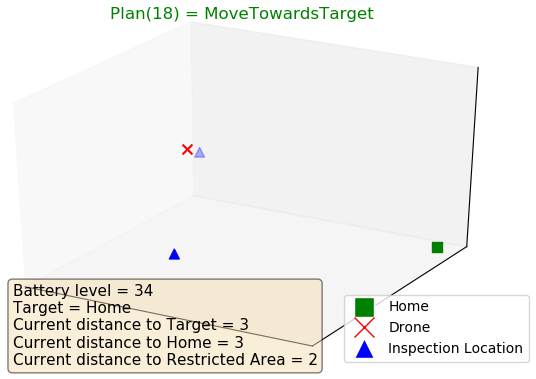
\includegraphics[width=0.5\textwidth]{plots/plt18}}
  \subfloat{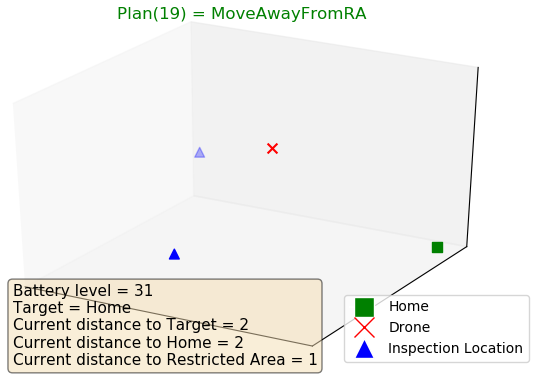
\includegraphics[width=0.5\textwidth]{plots/plt19}}
\end{figure}
\begin{figure}[!htb]
  \centering
  \subfloat{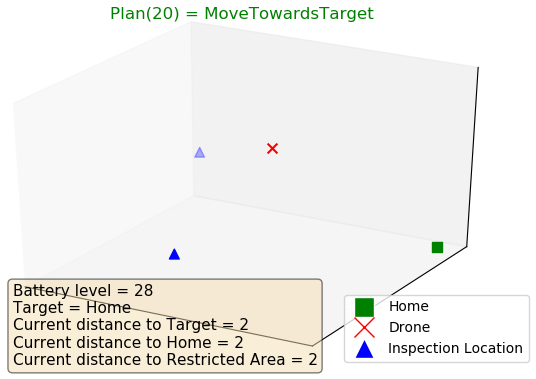
\includegraphics[width=0.5\textwidth]{plots/plt20}}
  \subfloat{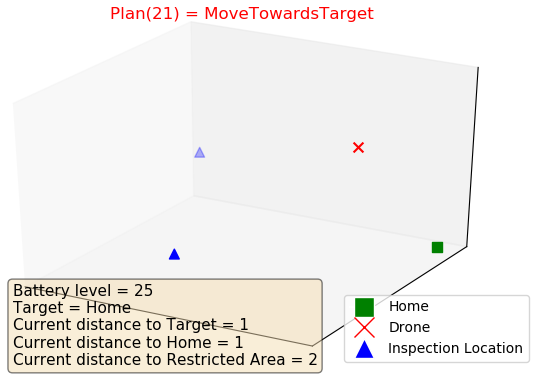
\includegraphics[width=0.5\textwidth]{plots/plt21}}
\end{figure}
\begin{figure}[!htb]
  \centering
  \subfloat{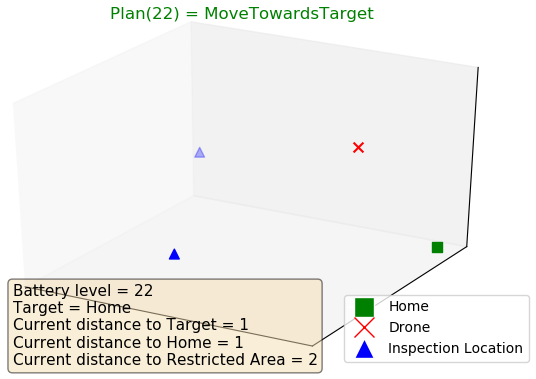
\includegraphics[width=0.5\textwidth]{plots/plt22}}
  \subfloat{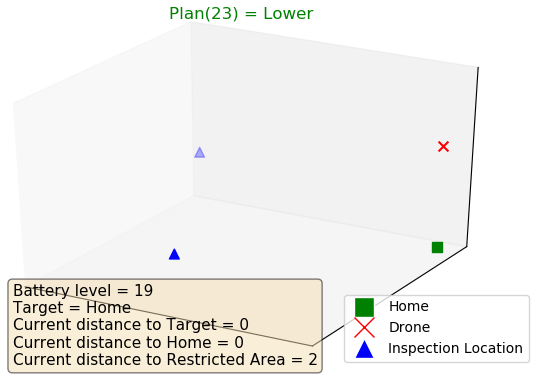
\includegraphics[width=0.5\textwidth]{plots/plt23}}
\end{figure}
\begin{figure}[!htb]
  \centering
  \subfloat{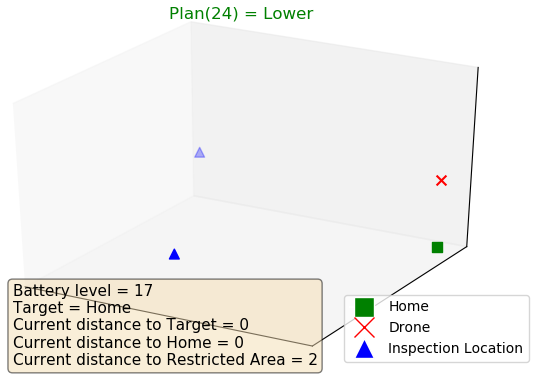
\includegraphics[width=0.5\textwidth]{plots/plt24}}
  \subfloat{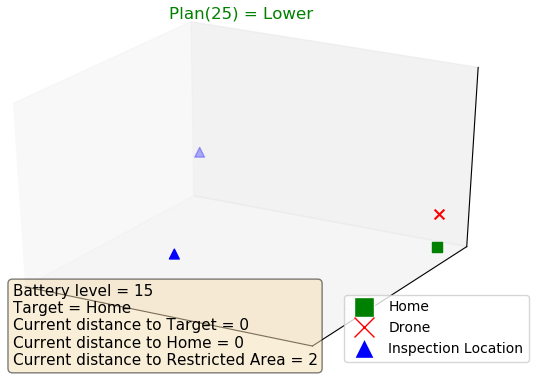
\includegraphics[width=0.5\textwidth]{plots/plt25}}
\end{figure}
\begin{figure}[!htb]
  \centering
  \subfloat{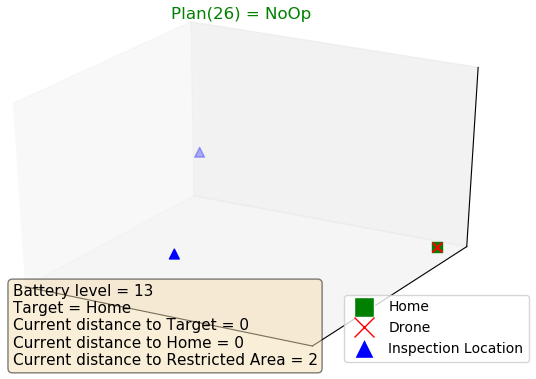
\includegraphics[width=0.5\textwidth]{plots/plt26}}
  \subfloat{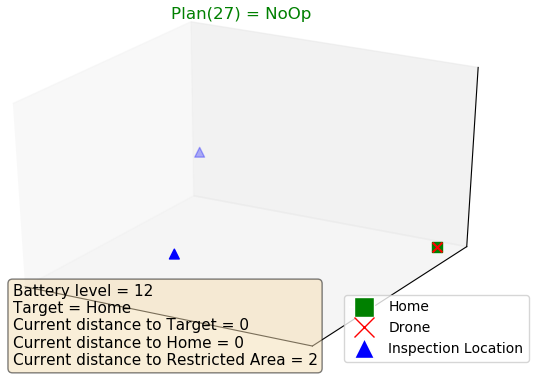
\includegraphics[width=0.5\textwidth]{plots/plt27}}
\end{figure}
\begin{figure}[!htb]
  \centering
  \subfloat{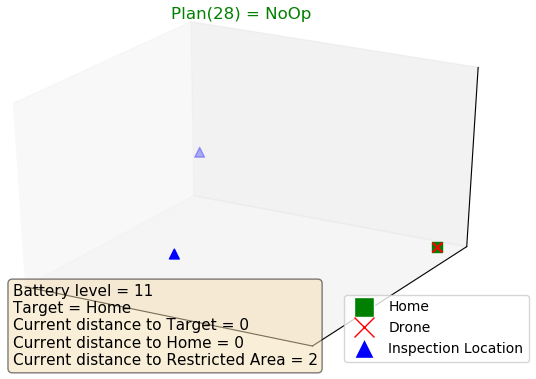
\includegraphics[width=0.5\textwidth]{plots/plt28}}
  \subfloat{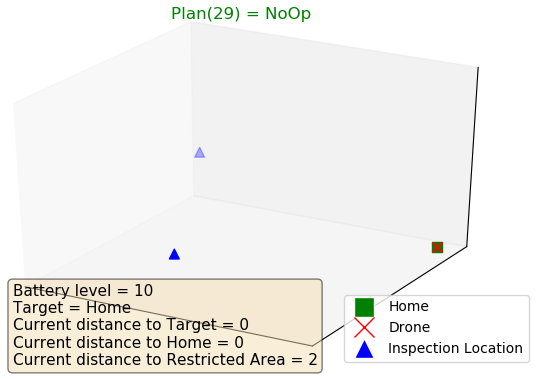
\includegraphics[width=0.5\textwidth]{plots/plt29}}
\end{figure}

\end{document}